\documentclass[12pt,letter]{article}
\usepackage[latin1]{inputenc}
\usepackage{amsmath}
\usepackage{amsfonts}
\usepackage{amssymb}
\usepackage{parskip}
\usepackage{xcolor}
\usepackage[margin=2.5cm]{geometry}
\usepackage{graphicx}

\newcommand{\QED}{
	\begin{flushright}
		\textit{\textbf{\#QED}}
	\end{flushright}
}

\begin{document}

Michael Beaver\\
CS 421, SP15\\
6 May 2015 \\
Lab \#4 
\hrule

\textbf{\S 5.1 7.} Find context-free grammars for the following languages (with $n \geq 0$, $m \geq 0$).

\textbf{\S 5.1 7c.} $L = \{ a^n b^m : n \neq 2m \}$\\
Note $m = 0 \Rightarrow n \neq 0$, so $\lambda \not\in L$.

$S \rightarrow aCb \ \ | \ \ a \ \ | \ \ b $\\
$C \rightarrow A \ \ | \ \ B$\\
$A \rightarrow aA \ \ | \ \ a \ \ | \ \ \lambda$\\
$B \rightarrow aB \ \ | \ \ b \ \ | \ \ \lambda$\\

\ \\
\ \\
\ \\

\textbf{\S 7.1 4.} Construct NPDAs that accept the following languages on $\Sigma = \{ a, b, c \}$.

\textbf{\S 7.1 4e}  $L = \{ a^3 b^n c^n : n \geq 0\}$\\
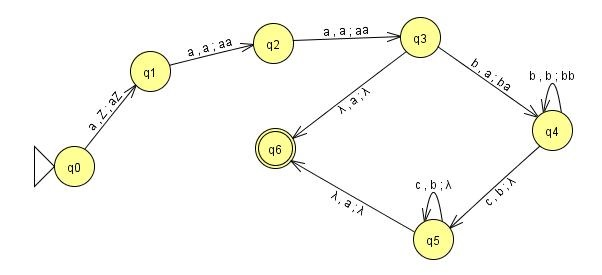
\includegraphics[scale=1]{714e.jpg}

\newpage

\textbf{\S 8.1 2.} Show that the language $L = \{ a^n : n$ is a prime number$\}$ is not context-free.

Assume $L$ is context-free and therefore pumpable with the Pumping Lemma for CFLs. Suppose we have a string $w = a^q$, where $q$ is a prime number such that $q \geq m$. We have that $w \in L$ and $|w| \geq m$. The string $w$ can then be subdivided in the following fashion: $w = a^r a^s a^t a^u a^{q-r-s-t-u}$. We see that $s + u \geq 1$ and $s + t + u \leq m$ satisfy our criteria for the Pumping Lemma for CFLs. We can pump $w$ to generate strings of the following form: 
$$w_i = a^r a^{si} a^t a^{ui} a^{q-r-s-t-u}$$
$$\Rightarrow w_i = a^{si + ui - s - u + q}$$
$$\Rightarrow w_i = a^{(s + u)(i - 1) + q}.$$
Now consider $i = q + 1$: $w_{q+1} = a^{(s+u)(q+1-1)+q} = a^{(s+u+1)q}$. Notice that $w_{q+1} \not\in L$ because $(s+u+1)q$ is not a prime number. Therefore, $L$ is not pumpable and is not context-free. \QED

\ \\
\ \\
\ \\

\textbf{\S 8.2 17.} Show that the language $L = \{a^n b^n : n \geq 0, n$ is not a multiple of 5$\}$ is context-free.

Let $L_1 = \{a^n b^n : n \geq 0\}$ and $L_2 = \{ a^n b^n : n$ is a multiple of $5\}$. We know that $L_1$ is not a regular language. We should be able to construct a finite automaton to accept $L_2$, so it should be a regular language. We can construct NFAs for $L_{2a} = \{a^n : n$ is a multiple of $5\}$ and $L_{2b} = \{b^n : n$ is a multiple of $5\}$. From here we can concatenate $L_2 = L_{2a}L_{2b}$ since regular languages are closed under concatenation. It is easy to see that $L = L_1 \cap \overline{L_2}$. Since $L_2$ is regular, $\overline{L_2}$ is also regular. Thus, we have the conditions for regular intersection, which is closed for CFLs. It follows then that $L$ is context-free. \QED 








\end{document}
